\section{ReportSection}
\label{sec:reportSection}

\begin{figure}[h!] 
	\centering
	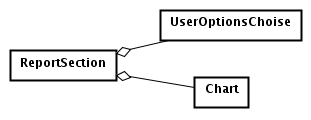
\includegraphics[width=0.5\textwidth]{../Milestone1-DomainModel/img/ReportSectionDetail.png}
	\caption{report section}
	\label{fig:reportSection} 
\end{figure}

Abbiamo da implemetare un requisito che vuole la possibilit\`a di aggiungere
alla reportistica un determinato \emph{Chart} con le relative \emph{UserOption}
scelte dall'utente. Modelliamo quindi il concetto di \emph{ReportSection} per
realizzare questo requisito. Come si vede dalla figura, \emph{ReportSection}
associa \emph{Chart} e \emph{UserOptionChoice}. Utilizziamo direttamente la
lista delle scelte\footnote{che viene costruita lato server} in modo da non
doverla costruire nella funzionalit\`a di assemblamento del report.
